\section{Introduction}
\subsection{Why study rulemaking?}
% \section{The Importance of Studying Rulemaking}
% Mobilization may increasingly target rulemaking because it is how most policy in the U.S. is now made. 
With the rise of the administrative state in the United States, federal agencies have become a major site of policymaking and political contestation. In the years or decades between legislative enactments, federal agencies make legally-binding rules interpreting and reinterpreting old statutes to address emerging issues and priorities. Ninety percent of new policy that carries the force of law is now made in the bureaucracy rather than in Congress \citep{West2013WhoControl}.\footnote{I use policy, law, and regulation as nested concepts. My methods generally apply to all policy texts whether they carry the force of law or not. Many public and private organizations, including agencies, have policy statements that are not legally binding. My empirical subject is rules that do carry the force of law based on some authorizing legislation. I use rule (a more technical term) and regulation (a more colloquial term) interchangeably.}
Examples are striking: %the effect of the Dodd-Frank Wall Street Reform and Consumer Protection Act was largely unknown until the specific regulations were written, and it continues to change as these rules are revised. 
Congress authorizes billions in farm subsidies and leases for public lands, but who gets them depends on agency policy. In the decades since the last major environmental legislation, agencies have written thousands of pages of new environmental regulations and thousands more changing tack under each new administration. This constant revision of administrative rules makes them distinct from legislation \citep{Wagner2017DynamicRulemaking}.
% And these revisions can be significant. In 2006, citing the authority of statutes last amended in the 1950s, the Justice Department's Bureau of Prisons proposed a rule restricting eligibility for parole. In 2016, the Bureau withdrew this rule and announced it would be requiring fewer contracts with private prison companies, precipitating a 50\% loss of industry stock value. Six months later, a new attorney general announced these policies would again be reversed, leading to a 130\% increase in industry stock value. %Like many rulemaking debates, industry and advocacy groups spent millions of dollars lobbying on this issue. Few rulemakings, however, receive this level of public and presidential attention. In the majority of rulemakings, few participate, and we do not really know the extent to which participants get what they lobby for.% (but see Yackee and Yackee 2006)
Rulemaking clearly matters.

Less clear, however, is what the new centrality of agencies and rulemaking means for the practice of American democracy. In addition to the complex relationships agencies have with the president and Congress, agencies have complex and poorly understood relationships with the public and advocacy groups. Relationships with constituents may even provide agencies a degree of ``autonomy'' from their official principals \citep{Carpenter2001}. While some suggest that requirements for agencies to solicit and respond to public comments on proposed rules allows ``civil society'' to provide public oversight, others note that participants in rulemaking often represent elite parts of society \citep{Seifter2016ComplementaryPower} and business interests \citep{Yackee2006a}. Yet agency decisions are also the target of protests and advocacy campaigns.\footnote{For example, along with 50 thousand protesters in Washington D.C., the State Department Received 1.2 million comments on the Environmental Impact Statement for the Keystone Pipeline. Similarly, along with the thousands of protesters supporting the Standing Rock Sioux protest to the Dakota Access Pipeline, the Army Corps of Engineers received hundred of thousands of comments. Along with 22 million comments on the Federal Communications Commission's Open Internet rules, activists are organizing online protest actions. On each of these issues, advocacy activity has been followed by legislative or executive action.} and the notice-and-comment process purports to be an avenue of citizen voice. Big red letters across the top of the Regulations.gov homepage solicit visitors to ``Make a difference. Submit your comments and let your voice be heard.'' A blue "Comment Now!" button accompanies a short description of each draft policy and pending agency action. While most rules receive little attention, the ease of online commenting and mobilizing has created exponential increases in the number of rules where which hundreds of thousands of citizens participate (see figure \ref{fig:comments}). Occasionally, large numbers of citizens are paying attention.

\begin{figure}[!hb]
\caption{Number of Public Comments Total (Left) and Under 1 Million (Right). The most commented on rules have been published by the Federal Communications Commission (FCC, omitted from this plot), the Environmental Protection Agency (EPA), the Department of Interior (DOI), the Bureau of Ocean Energy Management (BOEM), the Consumer Financial Protection Bureau (CFPB), and Fish and Wildlife Service (FWS).}
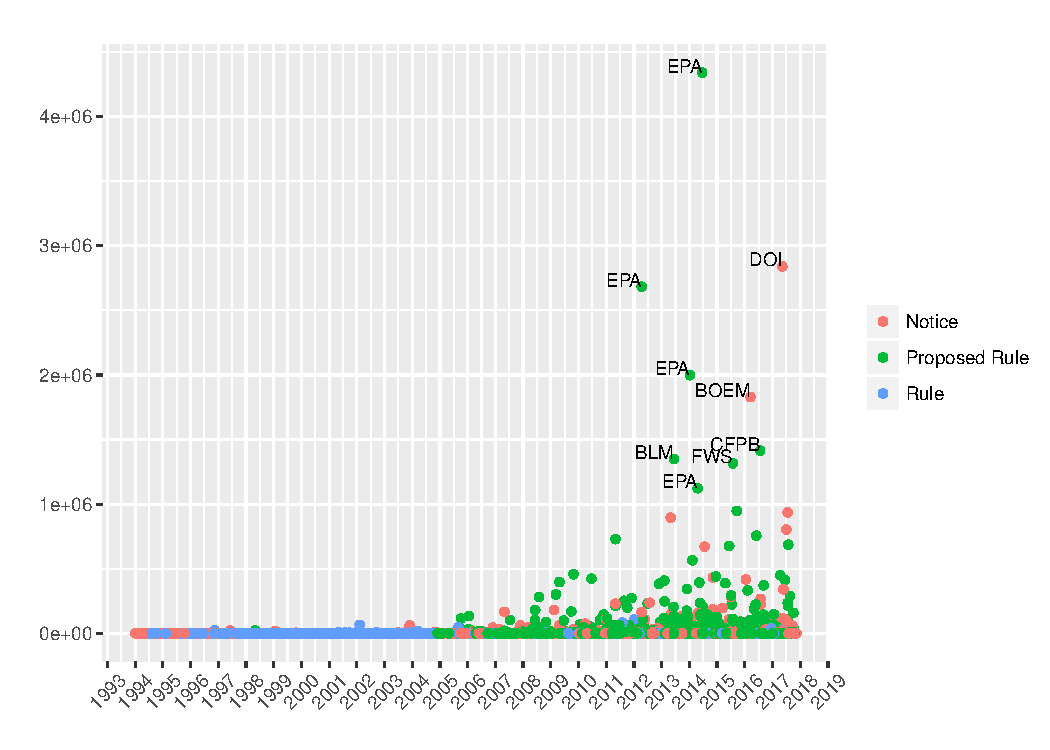
\includegraphics[width= 3.5in]{number_of_comments.pdf}
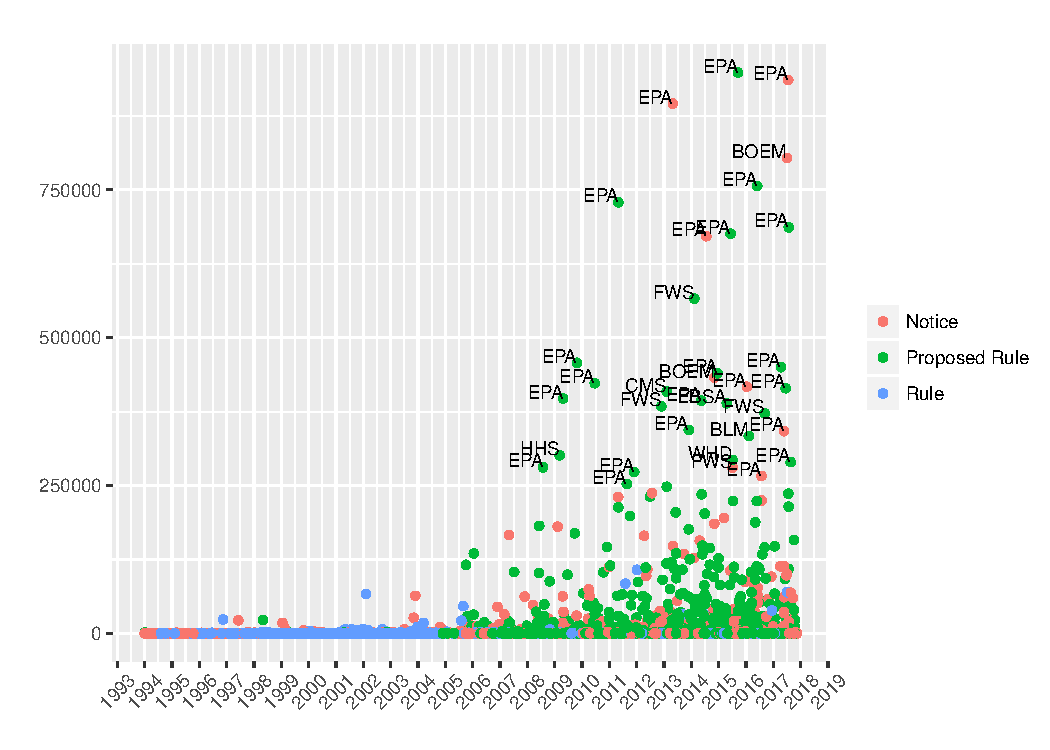
\includegraphics[width = 3.5in]{comments_under_1m.pdf}
\label{fig:comments}
\end{figure}

It is even less clear whether actions by average citizens make a difference in agency policymaking. Many may believe that they do, but the mechanisms are not obvious. Indeed letter writing and other forms of mass mobilization do not have a clear place in political scientists' theories of bureaucratic politics. This lack of scholarship may be the result of both a general suspicion, rooted in certain theories of strategic behavior, that mass politics affects unelected career officials as well as a normative assumption that policy ``implementation'' is no place for contentious politics. Neither the bureaucrat who asserts that rules are the result of scientific analysis nor the political scientist who asserts that rules are the result of bureaucrats strategically selecting their most preferred policy within institutional constraints offer an explanation for why an agency would receive millions of public comments or why they would matter.

In this 
dissertation,
% paper,
I argue that if we appreciate agency policymaking as a site of contentious politics, mechanisms emerge by which mass mobilization may affect both the strategic environment and ideological perspectives of those who write agency rules. While the theory that I assemble attempts to describe the relationship between mass mobilization and agency decisionmaking in general, my empirical focus is on the role of  organized campaigns targeting notice-and-comment rulemaking processes, with special attention to environmental 
%and financial 
regulation.



 \subsection{Puzzle: Why mobilize?}
% \section{Why mobilize?}

Prior to the 22 million public comments on the Federal Communications Commission's 2017 Open Internet rule,\footnote{It is yet unclear how many of these comments are from real people.} two of the most commented on rules set standards for mercury emissions from coal and oil-fired power plants. Among other things, the Environmental Protection Agency (EPA) solicited ``comments on whether there would be a basis for considering area sources to be significantly different from major sources,'' ``on the adequacy of the restrictions associated with bypass conditions regarding maintaining LEE status" and ``on the proposed revisions concerning [equations' 1a and 1b] usefulness in calculating the maximum potential emissions rate from an emissions averaging group'' (EPA 2011). LEE status is not defined in the notice soliciting comments, and equations 1a and 1b are surely inaccessible to most citizens. Yet these two proposed rules received 942,483 comments. 

One comment, from the United States Council of Catholic Bishops, read: ``While we are not experts on air pollution, our general support for a national standard to reduce hazardous air pollution from power plants is guided by Catholic teaching, which calls us to care for God’s creation and protect the common good and the life and dignity of human persons, especially the poor and vulnerable.'' Bishops are not known to closely follow power plant regulations. Their moral authority was mobilized by activists who wanted stricter regulation of mercury. Groups mobilizing on the mercury rules including environmental and health groups and industry competitors, including the owners of Nuclear, Natural, geothermal power plants. 

In the official, legally-required response to comments, the EPA did not discuss God's creation, dignity, or the poor.  Indeed, the EPA asserted that mercury levels are a matter of science, not not a matter of justice. But the EPA did implicitly assert a definition of the public good when it used studies of mercury's aggregate public health effects on the U.S. population to set emissions standard.\footnote{As Wagner (1995) %CITE
notes, ``agencies exaggerate the contributions made by science...in order to avoid accountability for the underlying policy decisions. Although camouflaging controversial policy decisions as science assists the agency in evading various political, legal, and institutional forces, doing so ultimately delays and distorts the standard-setting mission'' (p. 1617). She goes on to say that  ``While the APA mandates a process for public involvement, it provides almost no protections to ensure that agencies will explain the substantive bases for highly complex or technical rulemakings in a way that the lay public can readily understand and challenge'' (1656) and that ``Mischaracterization of the entire standard-setting endeavor as resolvable by science results in significant obstacles to democratic participation'' (1674). Similarly, Harvey Brooks (1984) notes that ``The modern nation risks being no longer recognizable as a democracy, either representative or plebiscitary, if more and more policy areas are excluded from public participation because of the technical complexity.''} 
Then, as required by the Supreme Court, it justified the same standards with cost-benefit analysis in a revised proposed rule, concluding that for every dollar spent to comply with the regulation, the U.S. public receives up to nine dollars in health benefits (EPA 2007). If this is how decisions are made, why did the EPA receive nearly a million letters? Why would citizen opinions matter? 

% Wagner: A variety of commentators have suggested that agencies may seek increased legitimacy or decreased political accountability by disguising their policy judgments as science. See Majone, supra note 18, at 15 ("Traditionally, government regulators have sought legitimacy for their decisions by wrapping them in a cloak of scientific respectability.");Roberts et al., supra note 26, at 120 ("Too many of the participants [in science-policy decisions] have good reasons not to distinguish scientific evidence from policy preferences, not to analyze carefully the various sources of technical disagreement, and not to accept responsibility for some decisions or judgments."). Beyond these common sense observations scattered at points in articles and books, there has been surprisingly little scholarly discussion of the comprehensive existence of or reasons for a science charade in regulation.

In contrast to the science-based objectivity presented by the EPA, political scientists, building on law and economics scholarship, offer a different theory of bureaucratic decisionmaking rooted in the policy preferences and strategic behavior of agency leaders and their political principals: Congress, the president, and the courts. They find that political principals do constrain agency action but also leave room for agencies to move policy toward their own ``ideal point.''\footnote{Though political scientists make diverse assumptions about what this ideal is and how to measure it.} Science may or may not inform preferences, but preferences and the power to realize them in a strategic environment are, these scholars say, are the proximate cause of policy. These scholars would see the Mercury Rules as the result of EPA officials writing a policy as close as possible to their ideal policy given their strategic constraints. 

But if the strategic model is correct, why write letters to the EPA? The EPA administrator has their preferences and the public has no direct power over their decisions. Why not write to the president or members of Congress who influence EPA's strategic calculations and are more directly accountable to public opinion? 

Other political scientists, along with scholars of public administration, organizational behavior, and sociology offer alternative theories that, while less parsimonious, squarely address how the process of soliciting and responding to public comments may influence agency policy. They find that agency staff develop relationships with those who regularly participate in policy processes: most often businesses but also professional associations and activist organizations. Relationships draw on and reproduce organizational identities and reputations. This scholarship has revealed a good deal about how organized groups lobby agencies and why they succeed, but it has yet to address why these groups sometimes mobilize thousands of citizens to write letters or protest agency decisions. The theoretical foundations for why mass mobilization may matter is underdeveloped and we lack empirical research on how it may affect agency policymaking. 

In this dissertation, 
%In this paper, 
I address this theoretical and empirical gap in our knowledge on the role of mass mobilization in bureaucratic policymaking. I expand and integrate the above theories to develop testable hypotheses and analyze rule-related texts %and field experiments 
to explore whether mass mobilization matters and, if so, why. 

I argue that if mass mobilization indirectly affects the strategic environment it does so by signaling grass-roots political power to elected officials and if mass mobilization directly affects agency policymaking it does so by evoking organizational identities and reputations. 
Like the vast majority of letter-writers, Catholic Bishops contribute little to the technical aspects of epidemiology, mercury regulations, or cost-benefit analysis. If they influence agency policymaking it is 
by signaling a threat of political backlash or 
by persuading bureaucrats directly that moving policy in a certain direction is the appropriate thing for the agency to do. 
The next two subsections address these indirect and direct mechanisms in more depth. A third discusses why we may still observe mobilization in the absence of influence. 
% Whereas social movement scholars and political scientists have focused the behavior of elected leaders, I focus on the latter pathway of direct persuasion. 

Precisely identifying who participates, how, and the dimensions of disagreement over time is key to any study attempting to discover whose ideas end up in policy. These are descriptive questions but they are not easy ones. In the empirical section, I address three descriptive questions: who participates, who lobbies together, and who wins\footnote{By \textit{who wins?} I mean whose ideas end up in policy. This is distinct from measuring \textit{influence} with respect to a counterfactuals or constellations of ideal points. I measure what people say they want and whether they get it. For example, I measure whether rules where commenters requested consideration of environmental justice issues were more likely to address environmental justice issues in the final draft}. Here, \textit{who wins?} is descriptive rather than causal. While insufficient to infer specific causal influence, policy moving in one's preferred direction may indicate that one is aligned with those who have power in that policy process. %There are many potential causes for policy outcomes matching certain policy demands, and I proposed field experiments to test several of them.
% \section{Mechanisms of Influence}

\subsection{Indirect Influence: Signaling a threat of backlash}
% \section{Theories and Case Selection}
Why might mass mobilization matter? The literature on bureaucracy offers two types of explanations rooted in either strategic behavior or organizational norms. Political scientists often focus on strategic context. Public administration and management scholars focus on organizational logics and identities. I begin with the ``indirect'' mechanisms that theories of strategic behavior suggest. 

In the U.S. context, there are three main mechanisms by which mass mobilization could affect an agency action by changing the strategic context. 
Mass mobilization may signal power to influence the responses to agency action from the White House, Congress, or courts. Many rules receive little attention from these other institutions, but all three significant powers to reward, sanction, or reverse agency actions \citep{Yaver2016}. 

% Arnold, Logic Of Congressional Action p 217:
% success depends in poat of the length and complexity of the causal chain connecting a policy instrument with its policy effects. When a causal chain is short and simple, citizens are more likley to know which policy instrument will produceth appropriate effects and are beter able to monitor the performance of their repre3sentatives,. When a causal chain is long and complex, or when a problem in society stems from multile causes, citizens may be incapable of doing the appropriate policy analysis and political anslyss ." 
% p 272 "resoonsiveness to both attentive and inattentive publics avaries depending on the procedures that govern how legislators requd their positions" 
% "The model of citizen's control that I have been discussing is essentially an auditing model. Citizens do not instruct legislators on how to vote, not do thay necessairlily have well-defined policy preferences in advance of cogressional action. Legialators neverthless have strong incentives to consider citizens' potential preferences when they are deciding how to vote for fear that making the wrong choice might triggger and unfavorable audit." 
% 


The White House has several tools to influence agency decisions \citep{Yackee2009a,Simon1954}. These executive orders \citep{Mayer1999}, appointments \citep{Doherty2014,Lewis2008,Wood1988}, budgets \citep{Whittington2003}, and review of proposed policies \citep{HAEDER2015InfluenceBudget,Acs2013}. 
Congress also has several tools to influence agency decisions. These include the power of the purse \citep{Fenno1986,Bolton2015}, oversight, and new legislation. Some research suggests that this constraint is larger under divided government \citep{Yackee2009b} and that under divide government Congress tends to divide power among multiple agencies \citep{Farhang2016}.
The anticipation of judicial review makes courts relevant to rulemaking. Some rules are also made under court-imposed settlement or with judicial deadlines. Judicial opinions may also call on Congress to act \citep{Yaver2017}.
Despite these mechanisms and because of conflicts among them, agency staff maintain significant power over agency decisions. For example, Congress is less assured of compliance when power is divided \citep{Yaver2016}.

% more good stuff
%\subsubsection{Legal Scholarship}
Legal scholars' case studies of specific rulemaking process offer an additional relevant body of research. Coglianese (1997) finds that litigation is a common extension of rulemaking. Indeed, unlike legislative lawmaking, rulemaking takes place in the clear and present shadow of judicial review (Rossi 2001). Stakeholders can challenge a rule in court on a variety of procedural grounds and on statutory interpretation. This scholarship suggests those who succeed in rulemaking are those with the resources and experience to succeed in court. Costly mass comment campaigns could be signaling the ability and willingness to spend resources to challenge the rule in court. 

Mass mobilization may signal political risks or benefits of engaging in agency policymaking to members of Congress and the White House. It also may signal to the agency that activists have the capacity to sustain pressure through the policy process \citep{Coglianese2001}, including challenging the policy in court, a constant threat agency policies. Thus, mass mobilization may act as a signal of political power that  reshape rule-writers' beliefs about their strategic context. 



\subsection{Direct Influence: Mobilizing identities and reputations}

I now turn to the direct-influence pathway: the ability of social movements to mobilize ideas, evaluative frameworks, and claims about what is appropriate and right that may affect bureaucratic decisions. %I use mobilization around the idea of ``environmental justice'' as an example where direct influence may be visible. 

Organizational theory suggests additional mechanisms by which mass mobilization may influence bureaucratic decisions more directly. Here the causal process involves mobilizing norms and ideas right and wrong rooted in individual and institutional identity. Because concepts of mission, reputation, and the validity of claims are intertwined, these mechanisms are difficult to precisely define. Nevertheless, scholars have identified several types of direct influence. One important factor in decision making is personal and institutional reputation \citep{Carpenter2001}. This can take several forms. For example, individuals trained as scientists and agencies that cultivate reputations for producing valid science may be persuaded by rigorous scientific claims. Similarly, individuals who identify strongly as public servants and agencies with reputations for public responsiveness may be persuaded by claims about public or "stakeholder" opinion. In general, claims that resonate with the problems an agency has been tasked with solving and the means it has to solve those problems are likely to be well received.  

% \subsubsection{ Agencies as Policymaking Venues}
% the good stuff
When political scientists ask whose interests and ideas become law, they have generally focused on the behavior of legislatures, how the executive branch drives legislation, and how the courts review it. Compared to legislative, executive, and judicial institutions, the administrative state is a recent development in American government and theory has not kept pace with the rise in bureaucratic policymaking. 

I argue that theories of bureaucratic policymaking have been characterized by constraining assumptions about what bureaucracies ought to do.  Normative assumptions that \citet{Wilson1967} identified half a century ago, and corresponding scholarly silos, have persisted. This has led to lines of research talking past each other and often failing to engage broader theories of policy change. In particular, I argue that the pervasive implicit assumption that bureaucrats ought to be neutral implementers implies that politics in agency policymaking is inherently undesirable, leading many scholars to focus on compliance with political principals and overlook the role participation and ideas. For example, scholars assume that agencies ought to be engaged in implementing legislation and executive orders. However, most rulemaking takes place many years or decades after its authorizing legislation under a different Congress and with little attention from the White House until the very final draft. Rules that do not follow from contemporary Congressional or executive priorities are often assumed to reflect bureaucrats going rogue or being captured by interest groups. Such studies suffer from a lack of attention to the complex political process of rulemaking. 

Accountability to elected officials has been central to the study of bureaucracy \citep{Epstein1999,Huber2002,McCubbins1984,Wilson1989,Potter2016Slow-RollingRulemaking,Lowande2018PoliticizationAgencies} %add Meier and O’Toole 2006; West 1995; Wood and Waterman 1994
Viewing agencies as \textit{agents} has prevented scholars from incorporating new insights about the endogenous relationship between policy and politics. I suggest rulemaking is better studied in the way that scholars study policymaking in specialized congressional committees than with an unrealistic dichotomy of sincere implementation versus capture or disloyalty. Normatively, accountability to political principals only one of several important concerns. Empirically, it is often unclear what accountability means and there is ample evidence that it may not be the primary driver of bureaucrat behavior.

In contrast to the dominant view of agencies as \textit{agents}, a growing literature in political science draws on scholarship in law and public administration as well as studies of agenda setting and lobbying in legislative policymaking to better understand agencies as policymaking bodies. Public administration and legal scholars have been more attentive to the prominent role of interest groups.  Kerwin (2003) notes that ``Interest groups could find few modes of government decision making better suited to their particular strengths than rulemaking.'' This research finds business groups to be most successful class of commenters in rulemaking \citep{Yackee2006a} especially when lobbying together, often, or unopposed (Nelson and Yackee 2012) and when lobbying across multiple venues \citep{Yackee2015}. Importantly, this literature notes that the currency of lobbying is information (Hall and Deardorf 2006), which includes both science and policy ideas \citep{Jones2005}. Kirilenko (2014) and Yackee and Yackee (2006) both find evidence that comments from sophisticated interest groups like businesses seem to influence rules. These scholars offer one set of answers to the question of who wins: those who succeed in rulemaking tend to be business interests, repeat players, those who lobby together, and those who lobby unopposed. They succeed because they bring in new voices and send unified messages at higher amplitudes, creating perceptions of political consensus.


%There may be an inverse relationship between how responsive agencies are to political principals and to the public \citep{Lewis}.

%Yet public administration and legal scholarship rarely address how interest groups gain political power in the first place. 

% more good stuff
A second major contribution to theory in this area is Carpenter's  research explaining bureaucratic autonomy \citep{Carpenter2001,Carpenter2012}. Rather than asking how bureaucratic practices fit with normative assumptions, he asks how agencies became independent policymaking bodies. Responding to principal-agent literature that has focused on the presidential and Congressional control, Carpenter finds much more complex sets of relationships that explain organizational power and behavior. One of the main tools he gives us for understanding the source of bureaucratic autonomy is the concept institutional reputations. Bureaucrats and the institutions they animate develop reputations for certain competencies: for example, for expertly adjudicating scientific claims, for effectively executing policy aimed at a given goal, or for divining the public interest. Reputations for expertise, effectiveness, or representativeness reflect the mixed roles assigned to the bureaucrats: advisors, implementers, and policymakers. 
% Like Carpenter, I call attention to the fact that agency policy shapes the coalitions that surround and influence it. I depart from Carpenter's narrative in that I do not focus on cases where agencies intend to have these effects. Whereas Carpenter is interested in how bureaucrats intentionally shape lobbying coalitions, I am interested in the endogenous relationship between policy and coalitions, intended or not. While not the focus of his study, Carpenter notes that relationships also evolve in unintended ways. 
%Policy may pro-actively recruit group support, but may also be reacting to political pressure \footnote{For example, an industry may successfully lobby to be reclassified to face lower pollution regulations, perhaps those faced by their competition, thus turning competitors into allies for future policymaking and increasing the size of the coalition for the lower standard.} or be an unintended side effect of action the agency sees as imperative.\footnote{For example, new science on the health hazards of mercury led to pollution controls that differentiated coal power plants and gas power plants reshaping coalitions by turning allies on former air quality policymaking into competitors in future rounds.} %Nevertheless, 
Carpenter and related scholars thus offer a second possible set of predictions for which movements are successful: those who succeed in rulemaking tend to be those with close relationships with the agency, conditional upon (and because of) how those relationships support the agency's reputation for expertise, competence, and representativeness. %Furthermore, lobbying coalitions, their relationship to the agency, and thus their success are functions of past agency policy. 

%Some scholars attempt to estimate the preferences of bureaucrats. Instead, I take 
% Carpenter's findings of close relationships between interest groups and agencies is a potential explanation for why some groups appear to have influence, i.e. because they are aligned with agency ideologies. As my core contribution is to assess how groups are empowered or disempowered rather than how agencies are empowered or disempowered, I focus on discovering which groups' comments are related to changes in rules regardless of whether this is what certain bureaucrats also wanted. 




% \subsubsection{Reputations for accountability, representation, equity, and expertise }

% [How specific organizational identities and reputations drive decisionmaking]

\subsection{Mobilizing for Recruitment}

A third possibility is that mobilization around bureaucratic decisions is unrelated to the possibility of affecting policy and primarily a way to recruit and engage members or raise the profile of the movement. If this is the case, behaviors like protesting and mass commenting on rules are largely epiphenomena to unrelated kinds of politics. Organizers may know that mobilization has minimal effects, but lead members to engage as means to other ends. Many of the mobilized themselves may doubt their efficacy but still take advantage of the opportunity to protest. 

% The remainder of this paper presents a case study and an empirical test of whether comments influences rulemaking.



[Elaborate on org behavior]

\subsection{Advancing Theories of Bureaucratic Policymaking}

Quantitative studies of bureaucratic policymaking in political science tend to collapse the time dimension and rarely consider the historical context in which each rule is made. For example, scholarship exploring how political context affects timing and delay in rulemaking models rules as if they are independent of each other and independent of the date they began (see Potter 2017). These studies also tend to focus on the degree to which agency policymaking reflects presidential, congressional priorities and, occasionally, interest group priorities. Political scientists most often ask if agencies are doing what the president wants, what congress wants, or something else. They find significant amounts of ``something else,'' but theory inconsistent on what it is and where it comes from. 

%bad stuff


\section{Methods}
This project makes two core contributions. First, I introduce new methods to 
%test theories about
measure the formation of lobbying coalitions, their demands, and whether they got what they asked for. 
% and of specific actors within coalitions
Second, I employ field experiments to test mechanisms by which mass mobilization may influence bureaucratic policymaking. 
%Rulemaking gives specific meaning to legislation and thus governmental force to political ideas. Like other policies, regulations also shape the terrain for future politics. 

\section{Measuring indirect influences}
To assess the direct influence pathway, I estimate the extent to which mass mobilization around bureaucratic actions makes members of congress or White House officials more likely to engage or react and whether such mass mobilizations is salient in subsequent litigation. 

Congressional attention to agency actions can be observed in several ways. Members of Congress who sit on oversight committees raise issues in oversight hearings, reports attached to each agency's budget appropriation, and in personal letters addressed to agency officials. Using text reuse methods I will identify when policy issues raised in draft rules and rule comments attract positive or negative attention from legislators. Using texts has several major advantages over previous measures of congressional attention and sentiment such as partisanship \citep{Yaver2016,Lewis2008}, changes in budget size, or the length of appropriations reports. Unlike partisanship, it is issue-specific and does not require assumptions about agency partisanship. While budget changes may reflect real costs, the many reasons that budgets change make it difficult to attribute changes to particular agency actions. The length of appropriations subcommittee reports may indicate the amount of attention committees pay to an agency but they do not vary significantly over time and do not indicate whether committee attention is positive or negative. 

[President and Secretary]

There are two ways to assess the courts as an indirect pathway where mobilization leads to influence. First, mass mobilization may increase the credibility of the threat of litigation. Second mass mobilization may influence the outcome of subsequent court cases over the rule. Both are difficult to measure. The first I measure with a combination of the litigation history of mobilizing groups and specific references to litigation in the comments. The second I assess by identifying instances where courts reference the number or direction of comments or other forms of protest in their decisions and compare rules to the rules under consideration in those cases. While this is rare, legal scholars have noted that " If the validity of a final regulation is challenged in court, the court's review will be based in significant part on how well the agency responded to the public's comments"  (Wagner 1995).

\subsection{Measuring Policy Change}
Policies may shape and be shaped by many forces, including the collective action of citizens, expert opinions, and businesses interests. Yet the drivers and consequences of policymaking are difficult to disentangle. Business groups may fund scientists or advocacy campaigns to preempt or undo costly regulations. Experts and policymakers may inspire broader civic mobilization, and citizen mobilization may, in turn, shape the priorities of experts and policymakers. Some policy debates divide along lines of citizen and corporate interest or expert and popular opinion, but many entail various clusters of claims regarding the public interest, expertise, and business interests: claims about the public good, scientific truths, and the proper role of government. Inferring policy demands from identity alone and assuming static coalitions may miss much of the story. 



\subsection{Data}
I focus on bureaucratic policymaking because, due to its sheer volume, it is both rich in opportunities to see different types of political mobilization, organization, and power at work and incompletely understood by political scientists. Specifically, I focus on agency rulemaking, a key part of U.S. policymaking that offers analytical leverage. Rulemaking is a process where agencies must solicit and respond to public comments on regulations (rules) before they carry the force of law (see Figure 1). Draft rules are published in a Notice of Proposed Rulemaking (NPRM). Occasionally, comments are also solicited before the draft rule is published through an Advanced Notice of Proposed Rulemaking (ANPRM). Intriguingly, while this process originally aimed to promote direct democracy and citizen voice, it is now generally seen as a mechanism to engage expertise (Coglianese 2006). Furthermore, research finds that the comment process actually favors business interests (Yackee and Yackee 2006). %Despite a large number of case studies, largely from legal scholars, our systematic understanding of the politics of rulemaking is thin.

% diogram of rulemaking  and commenting 
\begin{figure}[h!]
\label{inputs}
\caption{The Textual Record of Agency Rulemaking}
%\begin{table}
\begin{tabular}{@{\extracolsep{5pt}}cccccc}
 &  & &  \\
 & &\multicolumn{3}{c}{(Public Comments)}\\
 & & &$ \downarrow $& \\
\fbox{Inputs} & $\longrightarrow$ & \fbox{Proposal Text} &$\longrightarrow$ & \fbox{Outcome Text}\\
 & & & \\
List of Statutory Authorities &  & Proposed Rule & & Final Rule\\
(Advanced Notice)  &   &  & &   (and Response to Comments)\\
(Comments)  &   &  & &   \\
\end{tabular}
%\end{table}
\end{figure}
 

Rich data on several decades of rulemaking are available but have yet to be fully utilized by scholars.  Agencies publish draft rules, and comments received by interest groups, experts, and citizens. This offers leverage to identify the players, winners, and losers and to track those participating in the policy process over time. Rulemaking records often also cite the statutes, executive orders, and court cases that form a rule's historical institutional context. Some of this information, along with draft and final rule publication or withdrawal dates, is summarized since 1981 in the Unified Agenda of Regulatory and Deregulatory Actions (reginfo.gov). From 1994 onward, the text of most proposed draft rules, final rules, and summaries of comments received are published in the Federal Register (federalregister.gov). The result is the text of more than 70 thousand rules and . Finally, I collected text of over 7 million comments from 2002 onward via regulations.gov's API.

With the text of over 70 thousand regulations published since 1981 and over 7 million of the public comments on regulations since 2002, the second chapter of this dissertation will sketch the broad outlines of rulemaking in the American political context: who participates, how often rules are contested, whose ideas and interests are reflected in the text of rules, and who wins with different patterns of mobilization and contestation (or non-contestation). 

To make the project reasonable, the remaining chapters focus on [three] policy areas that have seen the highest levels of mass mobilization: [environmental, financial services, and communications technology]. To identify environmental rules, I select all rules made by the environmental protection agency and rules made by other agencies that cite president Clinton's executive order on environmental justice or president Obama's executive order on climate adaption. This allows me to consider how the same environmental problems may be addressed by different agencies. Financial services regulations are those that cite the Dodd-Frank act. Communications technology regulations are those proposed by the Federal Communications Commission.

%I also look closely at rules that end up before the Supreme Court. These rulemaking processes deserve extra attention for two reasons. First, regardless of how contentious they were at the rulemaking stage, these rules are key to understanding the nature and limits of executive power as a policymaking venue. Second, because all rulemaking is done in the shadow of judicial review, who wins in court and why shapes the political terrain of future rulemaking, empowering some groups with credible threats of litigation and disempowering others. References to court cases and implied threats of litigation are common in interest group comments, but to my knowledge, no study has looked systematically at how they affect rulemaking. Conversely, scholarship has not systematically assessed how mobilization and contestation in a rulemaking process affect judicial review. 